
\section{Analisi comparativa: controllo di posizione e di coppia ai giunti}
\label{sec:risultati_pos_vs_torque}

Per valutare le prestazioni dell'architettura di controllo proposta e la qualità dell'inseguimento della traiettoria di evasione, è stata condotta un'analisi comparativa tra due diverse strategie di controllo a basso livello descritte nella Sezione~\ref{subsec:controllo_posizione}:

\begin{itemize}
	\item \textbf{Controllo di posizione ai giunti}: la traiettoria cartesiana viene convertita nello spazio dei giunti ed inviata direttamente al controllore di posizione interno del robot. Sebbene tale schema presenti un'elevata semplicità computazionale, la natura discreta dei riferimenti generati esternamente al loop a $1\text{ kHz}$ rende il sistema sensibile a minime discontinuità o ritardi di sincronizzazione. Come evidenziato dai risultati sperimentali riportati in Figura~\ref{fig:velocitgiuntirealepc}, ciò si traduce in accentuati picchi nelle velocità di giunto e nell'insorgenza di rumore ad alta frequenza (\textit{jitter}), penalizzando la fluidità del moto.
	
	\item \textbf{Controllo di coppia ai giunti}: la legge di controllo calcola direttamente le coppie da applicare ai giunti integrando un regolatore Proporzionale-Derivativo (PD) con compensazione della dinamica. Questo approccio introduce un'azione di filtraggio intrinseca che smussa le variazioni brusche dei riferimenti, garantendo un'uscita intrinsecamente più regolare. I risultati in Figura~\ref{fig:jointspeedcompensatedtc} mostrano una drastica riduzione del \textit{ripple} e la completa eliminazione dei picchi di velocità, assicurando un profilo di moto continuo e una maggiore stabilità operativa dell'intero manipolatore.
\end{itemize}

\begin{figure}[htbp]
	\centering
	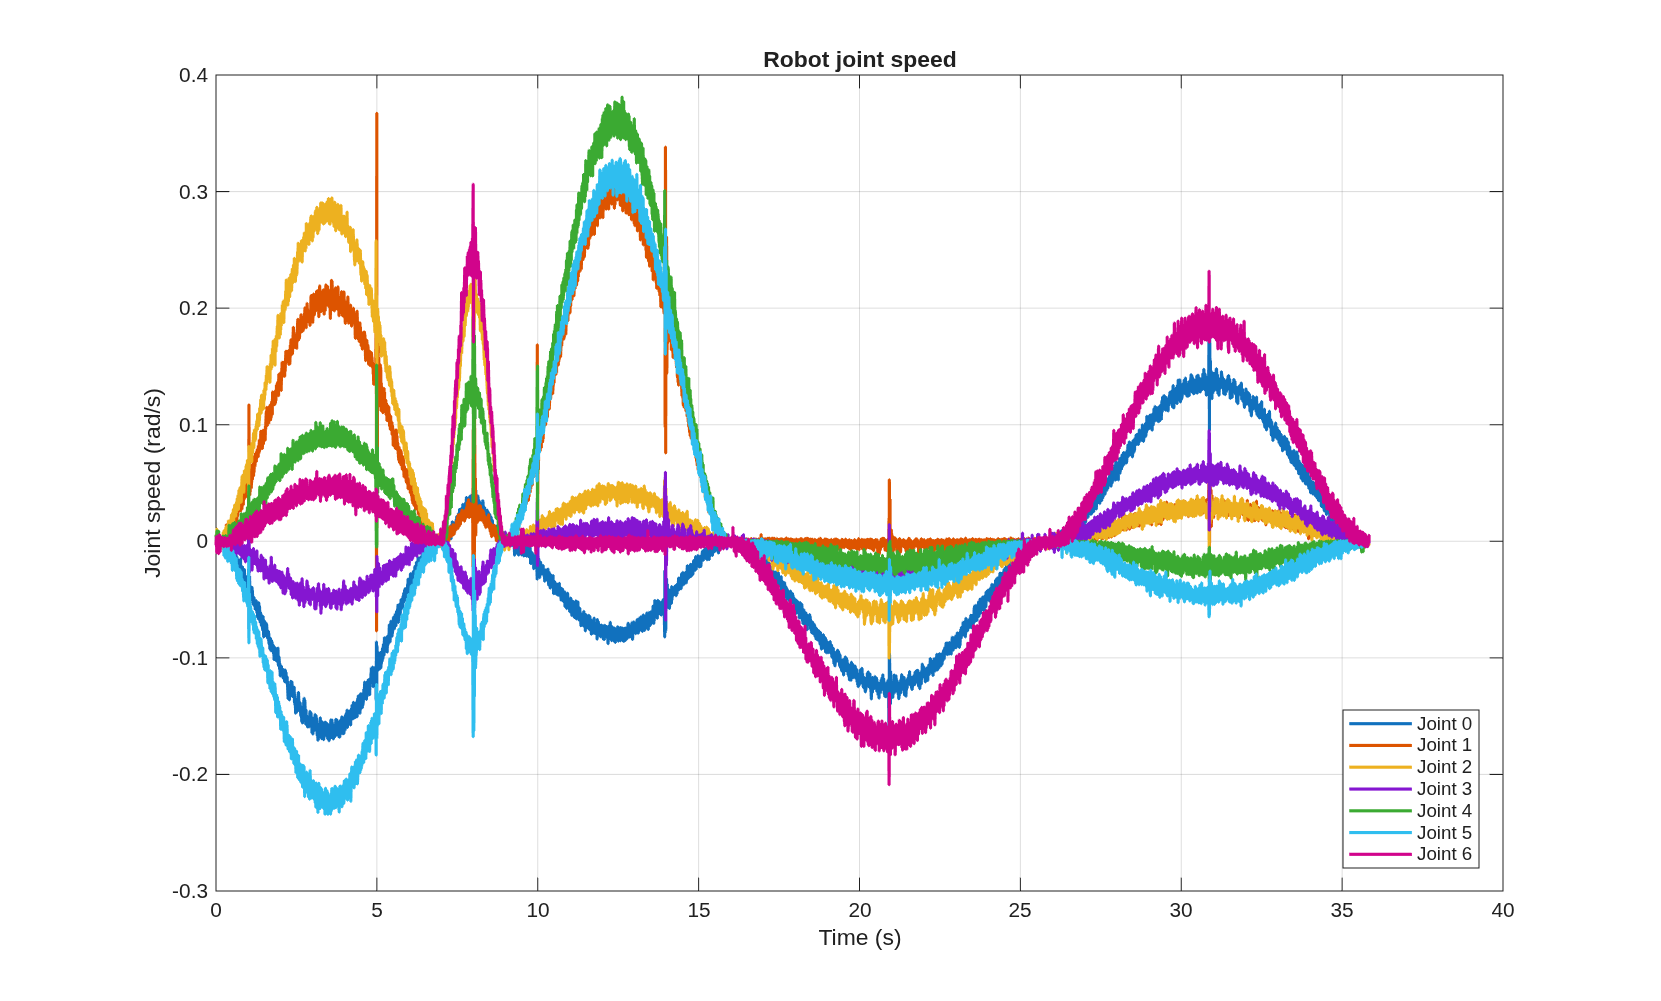
\includegraphics[width=0.85\linewidth]{figure_tesi/velocit_giunti_reale_PC}
	\caption{Profilo delle velocità ai giunti registrato con l'adozione del controllo di posizione. Si notino i picchi impulsivi e il fenomeno di \textit{jitter} dovuto alle discontinuità dei riferimenti.}
	\label{fig:velocitgiuntirealepc}
\end{figure}

\begin{figure}[htbp]
	\centering
	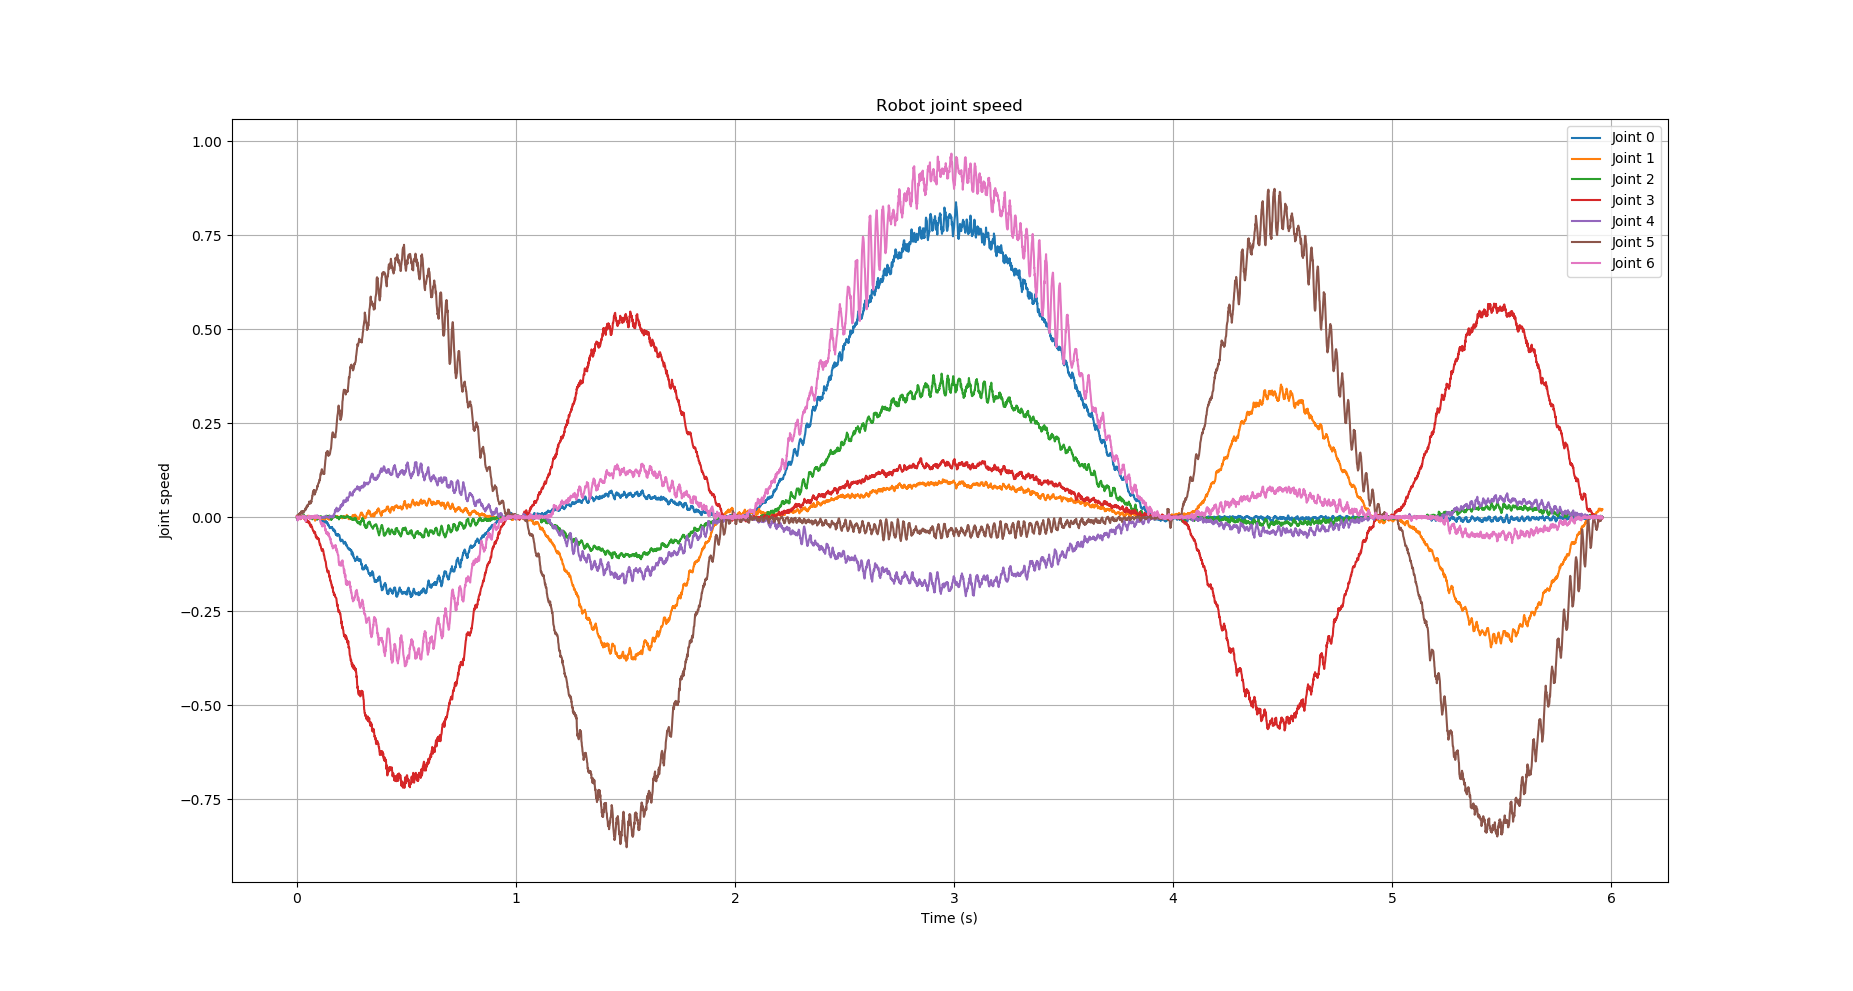
\includegraphics[width=0.85\linewidth]{figure_tesi/joint_speed_compensated_TC}
	\caption{Profilo delle velocità ai giunti con schema di controllo di coppia guidato dal regolatore PD. L'azione del controllore elimina i picchi, garantendo un'andamento fluido e privo di \textit{ripple}.}
	\label{fig:jointspeedcompensatedtc}
\end{figure}


\section{Risultati del primo approccio: arresto ottimizzato con capsule dinamiche}
\label{sec:risultati_primo_approccio}

Per valutare il comportamento del primo approccio di sicurezza, la metodologia è stata testata durante l'esecuzione di un compito nominale di \textit{pick-and-place}. Nel corso della traiettoria, al tempo $t \approx 2.5\text{ s}$, è stato introdotto un ostacolo virtuale mobile al fine di simulare un'intrusione nello spazio di lavoro e generare un evento di arresto di emergenza.

I risultati sperimentali, illustrati nelle Figure~\ref{fig:speedcalibrated1stoptc}, \ref{fig:duration1stoptc} e \ref{fig:raggicapsule1stoptc}, evidenziano i seguenti aspetti fondamentali:

\begin{itemize}
	\item \textbf{Profilo delle velocità ai giunti} (Figura~\ref{fig:speedcalibrated1stoptc}): alla ricezione del segnale di stop ($t \approx 2.5\text{ s}$), il controllore comanda una decelerazione fluida e continua, invertendo temporaneamente il verso del moto per riportare il robot verso la posizione iniziale in sicurezza, fino al completo azzeramento delle velocità di giunto.
	
	\item \textbf{Ottimizzazione online dei tempi di arresto} (Figura~\ref{fig:duration1stoptc}): la durata della frenata ottimizzata $T_{\text{stop}}$ viene ricalcolata continuamente in funzione dello stato cinematico istantaneo. In condizioni di velocità elevata, il valore stimato converge verso il limite superiore impostato ($0.4\text{ s}$), mentre al ridursi della velocità si attesta sul valore minimo di sicurezza ($0.25\text{ s}$).
	
	\item \textbf{Adattamento dinamico dei volumi delle capsule} (Figura~\ref{fig:raggicapsule1stoptc}): le dimensioni delle capsule di protezione si ridimensionano in tempo reale rispecchiando fedelmente il profilo del tempo di stop $T_{\text{stop}}$, espandendo il volume di inviluppo durante le fasi ad alta energia cinetica e riducendolo progressivamente durante la decelerazione.
\end{itemize}

Piccole asimmetrie o lievi sfasamenti temporali osservabili tra l'andamento delle velocità e le curve dei tempi di stop sono riconducibili all'architettura software multi-thread. Per garantire in modo deterministico la frequenza di aggiornamento di $1\text{ kHz}$ dell'anello di controllo di basso livello del manipolatore, l'algoritmo di ottimizzazione e il modulo di rilevamento degli ostacoli vengono eseguiti in modo asincrono su un thread dedicato a priorità distinta.

\begin{figure}[htbp]
	\centering
	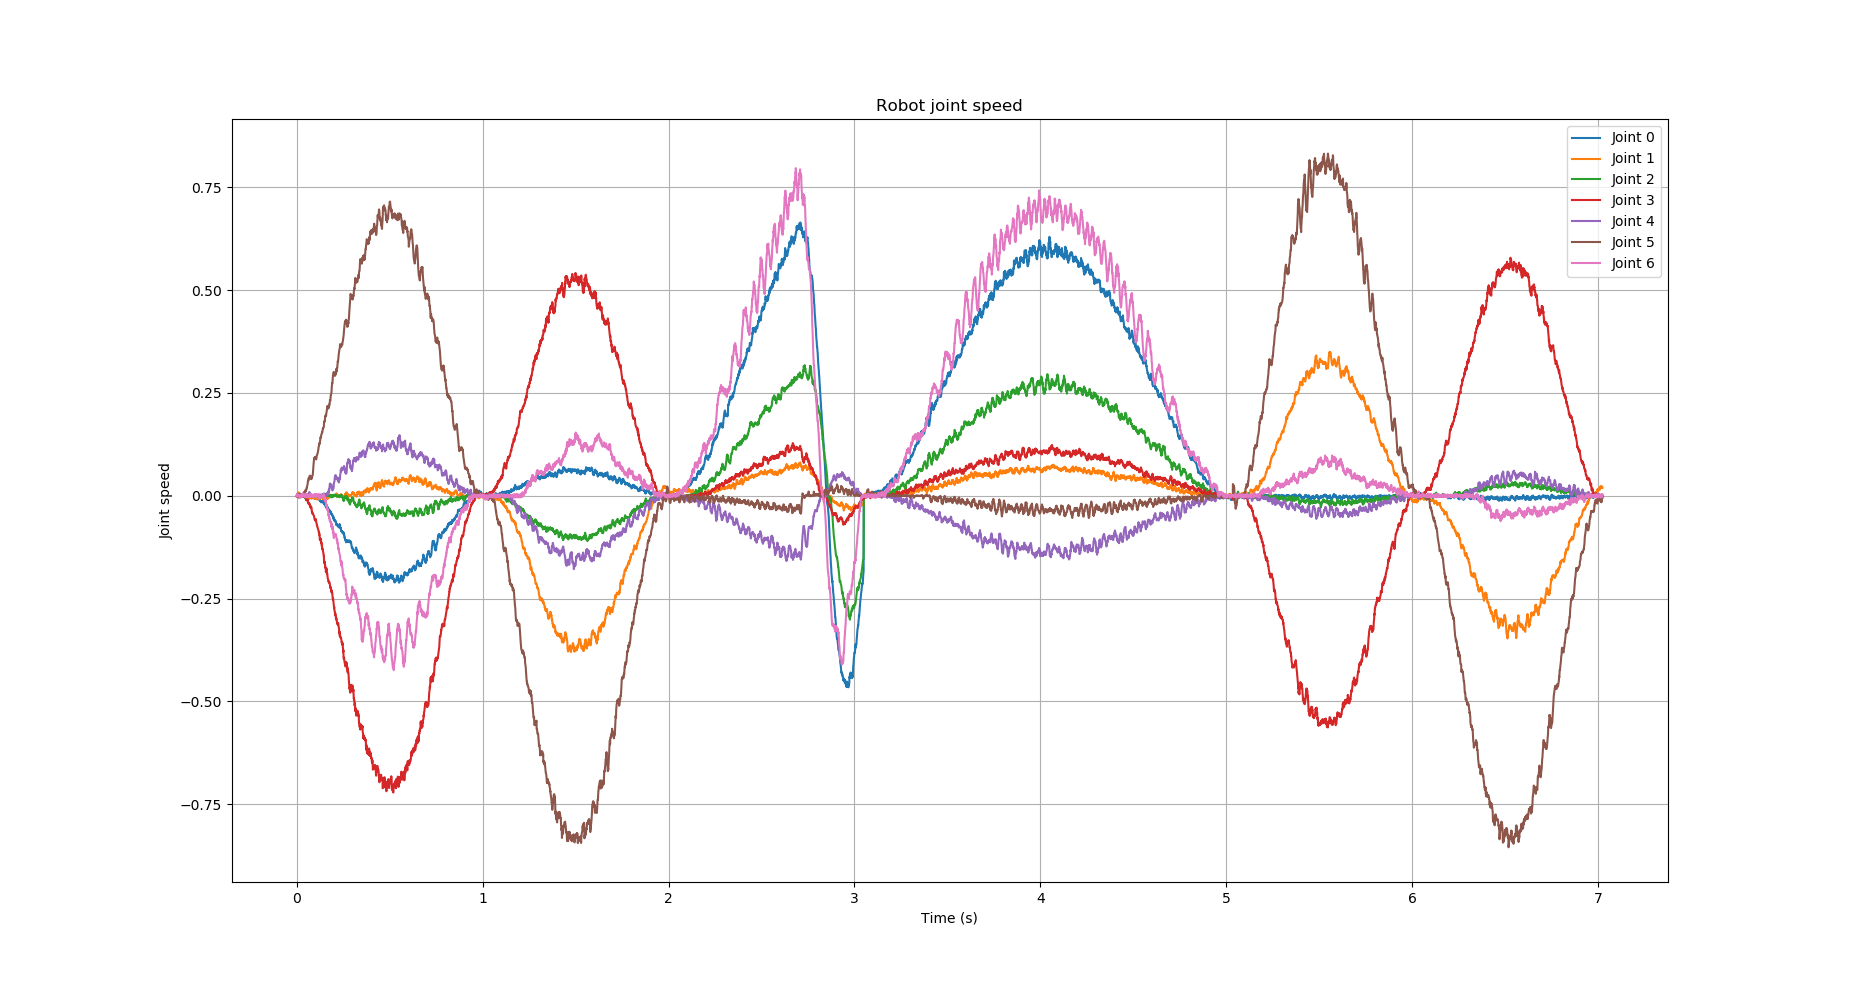
\includegraphics[width=0.85\linewidth]{figure_tesi/speed_calibrated_1stop_TC}
	\caption{Profilo temporale delle velocità ai giunti durante la traiettoria di \textit{pick-and-place}. Al tempo $t \approx 2.5\text{ s}$ viene rilevato l'ostacolo e attivata la procedura di arresto continuo.}
	\label{fig:speedcalibrated1stoptc}
\end{figure}

\begin{figure}[htbp]
	\centering
	
\includegraphics[width=0.85\linewidth]{figure_tesi/duration_1stop_TC}
	\caption{Andamento del tempo di arresto ottimizzato $T_{\text{stop}}$. Si nota la modulazione continua tra il valore minimo ($0.25\text{ s}$) e massimo ($0.4\text{ s}$) in base alla velocità istantanea.}
	\label{fig:duration1stoptc}
\end{figure}

\begin{figure}[htbp]
	\centering
	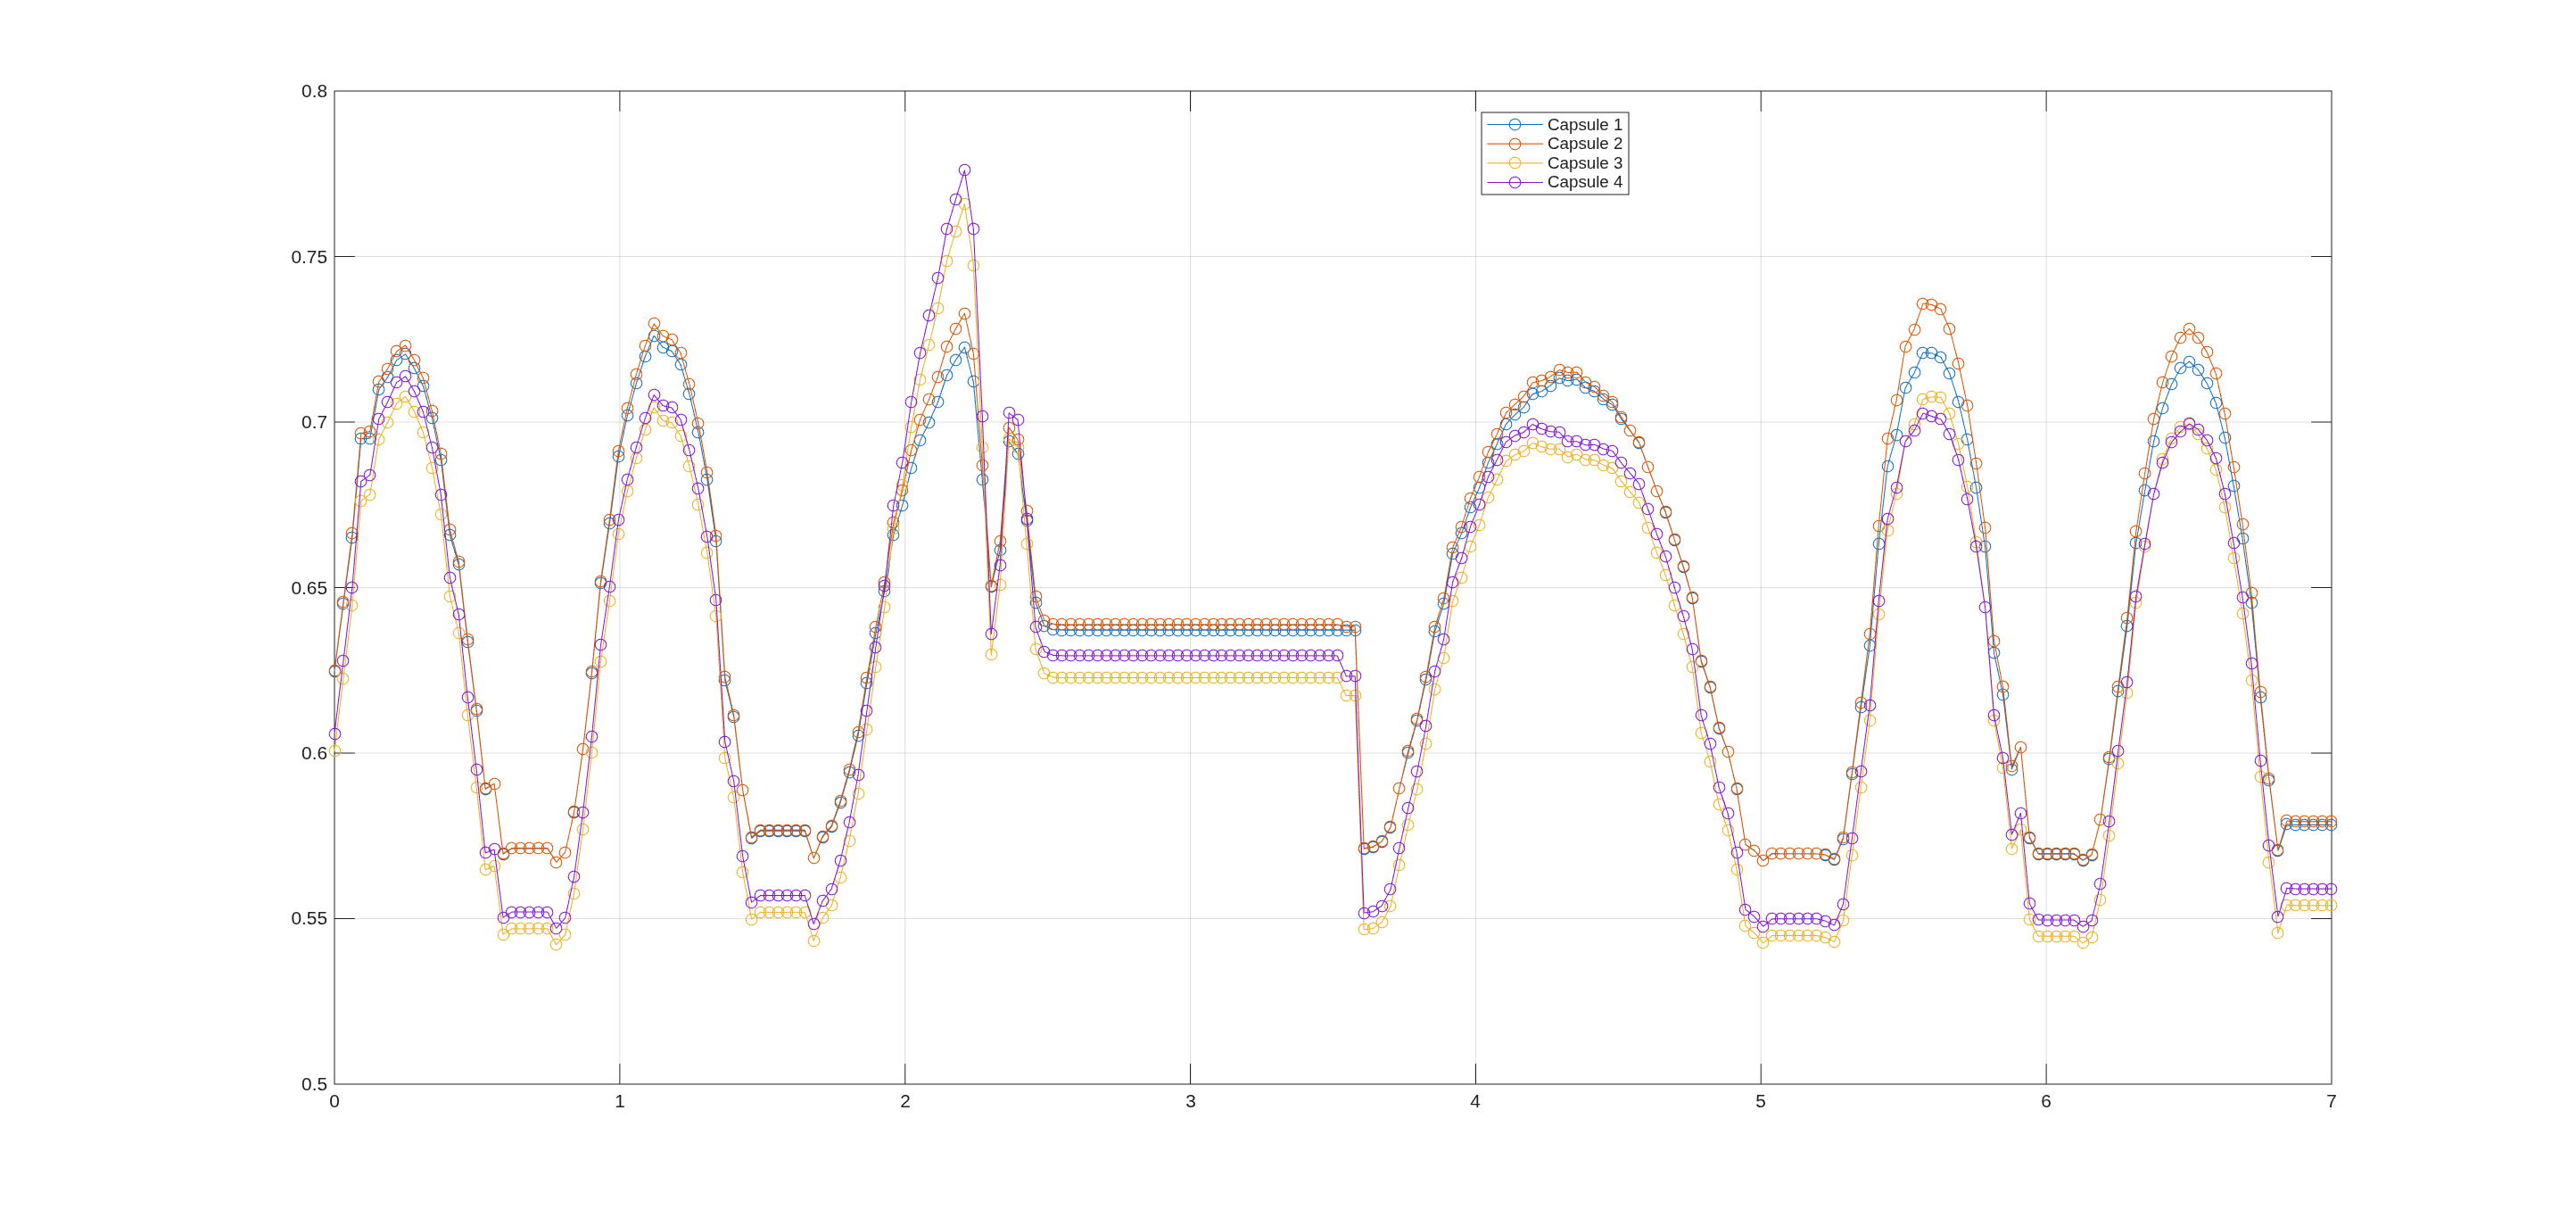
\includegraphics[width=0.85\linewidth]{figure_tesi/raggi_capsule_1stop_TC}
	\caption{Evoluzione temporale dei raggi delle capsule di protezione dinamiche, coerente con il profilo di decelerazione del robot.}
	\label{fig:raggicapsule1stoptc}
\end{figure}




\section{Secondo approccio}

\section{Contronto metriche di fluency}